\chapter{Introduction}

\section{Chromopainter and ancient DNA}

In this introduction I will discuss the following points: i) What are `haplotype-based' methods and what advantages and disadvantages do they offer over `unlinked' methods, ii) a summary of different methods used to analyse ancient DNA and iii) the need to merge datasets genotyped on different arrays. 

\subsection{Gains to be made with haplotype information}

\subsubsection{History}

Haplotype-based methods are statistical approaches in genetic analysis which explicitly model linkage disequilibrium (LD), or the correlation in frequency, between neighbouring genetic markers along a haplotype \footnote{Note that other methods, for example \texttt{octopus} \cite{octopus} are referred to as `haplotype-based' genotype callers, but they represent a distinct group of methods to e.g. ChromoPainter.}. This is in contrast to `unlinked' methods, which assume a model of linkage equilibrium between SNPs. A `haplotype' is a contiguous sequence of alleles which are located on the same chromosome. In this thesis, I will concentrate on haplotype-based methods in the context of identifying shared haplotypes between individuals in order to understand the genetic structure and history of a population(s).    

Linkage disequilibrium (LD) is the key concept underpinning haplotype-based approaches. It has been studied since the earliest days of genetics \cite{morgan1912complete, bateson1902experiments} and has since been a fundamental aspect of virtually all areas of genetics \cite{slatkin2008linkage}. The primary advantage of accounting for LD in a model is that information about the frequency of an allele in a population also provides  information about the frequency of neighbouring alleles within the same population. 

Some of the earliest uses of LD information for the study of genetic structure came from microsatellite markers, whose linked tandem repeats can be thought of as analogous to linked alleles on a haplotype. Microsatellites were, and still are, commonly applied to study the population structure of wild animal systems; for instance, Amos et al (1993) used microsatellites markers to examine the population structure of whales \cite{amos1993social}. Later, microsatellites at the CD4 locus were leveraged to show the preferred model of Human population history was a recent African origin \cite{tishkoff1996global}. This was deduced as Sub-Saharan Africans had substantially more variability in haplotype frequency and a higher diversity of STRP alleles associated with the Alu deletion than non-Africans, strongly suggesting Africa was the common origin of these haplotypes. This study outlined the insights into population history that can be obtained from the analysis of a very small number of linked markers.  

The next major advance was the development of methods to use LD information between SNP markers rather than within microsatellites, as SNPs are substantially more numerous across the human genome. Studies in the early 2000s utilised the then-new Hap-Map results \cite{gibbs2003international} to show LD varies across the human genome \cite{crawford2004evidence} and between worldwide populations \cite{evans2005comparison, reich2001linkage}, and that such variation can be used to make inferences about human populations history \cite{conrad2006worldwide}. Using 3,024 autosomal SNPs, Conrad et al (2006) calculated the proportion of unique haplotypes that were shared between two geographic regions, and by showing that the number of distinct haplotypes per region declines from Africa, provided additional evidence to support the previously proposed recent African origin of humanity \cite{cann1987mitochondrial}. It was also shown that isolated Native American populations had approximately 3 times fewer haplotypes per genomic region, indicating that recent endogamy plays a large role in shaping patterns of haplotype variation. 
 
The 2000s also saw a rapid increase in the number of SNP markers and individuals which had been sequenced. Accounting for LD and recombination within a model is necessarily computationally complex and the number of combinations of alleles and their possible evolutionary histories balloons as the number of loci increases. Therefore, the new era of sequencing demanded new and more efficient methods to cope with such data. The development of the Li and Stephens copying model (LSM) \cite{Li2003} was instrumental in the development of such methods \cite{song2016li} and provided an elegant solution to the increased complexity when modelling recombination between linked loci. As such, it has since played a part in virtually all areas of genomic methodology; for example, the LSM was, and still is, the foundation for methods of the haplotype phasing methods needed for haplotype-based methods \cite{stephens2003comparison, stephens2005accounting}.  LSM provides a way to generate a `target' haploid conditional upon a set of other observed haploids, specifically by modelling it as a `mosaic' of  the other sampled haploids using a Hidden Markov Model. The conditional probability that the target haploid `copies' from a particular reference haplotype is obtained by observing whether the alleles at the same position match between the target and reference haplotypes. The mosaic nature of the target haplotype reflects how historical recombination alters the genealogy relating sampled haplotypes along a genetic sequence, which in this model causes so-called `switches' in which reference haplotype it copies from. In general, if a target haploid matches a DNA segment to a particular reference haploid for a genomic region, the target is inferred to share a most recent ancestor with that reference haploid, relative to all other reference haploids, for that genomic region.

The first paper to use the LSM model explicitly to study human population history was that of Hellenthal et al 2008 \cite{hellenthal2008inferring}. The original LSM was developed to infer recombination rates. It did so by randomly ordering a set of phased haploids, presumed to be sampled from a genetically homogeneous population, and then taking each haploid in turn and forming it as a mosaic of the haploids earlier in the random ordering. They then multiplied the resulting probabilities of generating each haploid, using this so-called ``product of approximate-conditional'' (PAC) likelihoods as a basis to infer the recombination rate. Hellenthal et al 2008 instead used the mosaic approach to calculate the probability of forming a set of haploids from one population as a mosaic of those from another population(s), using these probabilities to infer the relative order in which populations were formed. While their approach had some flaws, such as not explicitly accounting for admixture, it provided some insights into the power of LSM-based approaches to infer features of human history, using only a modest number of SNPs (n=2,560). For example, similar to the results of Conrad et al (2006), Hellenthal et al's analysis of the structure of global haplotype sharing provided strong evidence of a recent African origin of modern humans. In the same year, Jakobsson et al (2008) analysed a much larger number of SNPs (n=525,910) and 29 worldwide populations \cite{jakobsson2008genotype} to show that haplotype clusters show an elevated ability to determine local structure compared to unlinked SNPs alone;  51\% of haplotype clusters were found in at most two regions, in contrast with 4\% of SNP alleles. 

Building on the copying model proposed by Hellenthal et al (2008), Lawson et al (2015) \cite{Lawson2012} created ChromoPainter, again based the LSM. ChromoPainter is a more general model than that of Hellenthal 2008; whereas the Hellenthal 2008 model was explicitly formulated to determine the ordering of human colonisation, ChromoPainter efficiently forms a set of target haplotypes as a mosaic of a set of reference haplotypes. In particular, it generates a `coancestry matrix', which gives information on the level of recent shared ancestry between each donor and recipient individual. ChromoPainter also allowed for the user to input recombination rate maps containing estimated recombination rates between neighbouring SNPs. Analysis of simulated data showed it to have an enhanced ability to separate closely related populations when plotted on a PCA compared to unlinked methods. It was developed in tandem with its own clustering method fineSTRUCTURE, and has since been extended into methods to detect and date admixture \cite{Hellenthal2014}, and infer ancestry proportions \cite{Hellenthal2014,Chacon-Duque2018}. 

The `next-generation' of chromosome painting methods had to confront the same issue that Li and Stephens did, which was how to adapt methodology to larger and larger sample sizes. ChromoPainter was designed with datasets of <10,000 people in mind, whereas biobank-scale datasets typically contain 500,000+ individuals. As such, ChromoPainter does not scale well to large datasets, especially when there are a large number of donor haplotypes. 

One approach is to use the Burrows-Wheeler transform (PBWT) \cite{burrows1994block, DurbinPBWT} to efficiently find matching haplotypes in large datasets. The insight to apply the PBWT to genetic data has been one of the most crucial insights into computation biology, as it allows for substantial increases in efficiency across a wide range of applications such as sequence alignment \cite{LiBWA}, phasing \cite{delaneau2018integrative} and data compression \cite{naseri2019multi}. PBWT has been applied to Chromosome Painting on Biobank-scale datasets in several recent papers \cite{byrne2020dutch, saada2020identity}. Similarly, methods to detect IBD in Biobank-scale cohorts have leveraged the PBWT \cite{naseri2019rapid, zhou2020fast}. However, PBWT-based approaches are still relatively immature; for example, they do not allow for the use of a reference panel and all haplotypes must be compared to all other haplotypes in an `all-v-all' manner (further explanation given in Appendix section \ref{sec:allvall}). Despite their current limitations, it seems that the future of Chromosome Painting will at least in part be based on the PBWT or similar approaches that increase computational efficiency, even if at slight losses in accuracy. Byrne et al used ChromoPainter and PBWT-paint to a subset of Dutch individuals and found eigenvectors of the coancestry matrix to be almost identical ($r^2 = 0.99$) and the correlation between raw coancestry matrices to be lower at ($r^2 = 0.82$).

\subsubsection{Advantages of accounting for haplotypes}

ChromoPainter can be run in either `linked' or `unlinked' mode. In the linked mode, described in detail in sections \ref{sec:ChromopainterDescription}, LD between neighbouring SNPs is accounted for. Unlinked mode assumes a model of linkage equilibrium between markers and has been shown to be statistically identical to the likelihood model underlying the commonly used ADMIXTURE algorithm \cite{Lawson2012}.

A typical case study, and one which I will return to in later chapters, was a study investigating population structure among individuals from the British Isles \cite{Leslie2015}. This study, hereafter referred to as POBI, genotyped 2039 people from England, Wales and Scotland \cite{Leslie2015}. One finding was that it was possible to detect structure between individuals from Devon and Cornwall (two neighbouring counties) using ChromoPainter. On the other hand, this structure was not discernible when using unlinked methods (PCA). This outlines the benefits of incorporating linkage information when attempting to identify fine-scale structure between closely related groups of individuals.

Gattepaille and Jakobson (2012) \cite{JakobssonCombiningMarkers} provided the mathematical foundations for the advantage of using linked markers over unlinked ones. They describe a metric, $GIA$ (gain of informativeness for assignment), a term borrowed from information theory, to describe the additional amount of information gained when using haplotype data instead of unlinked alleles. They showed that whilst combining two markers in linkage equilibrium is not necessarily advantageous for ancestry inference, $GIA$ is often positive for markers in LD with one another, demonstrating the advantage of haplotypes. Under a variety of simulated scenarios, incorrect assignment of individuals into populations was reduced between 26\% and 97\% when using haplotype data. For example, they showed that using empirical data of individuals from France and Germany, accounting for haplotypes could reduce the rate of mis-assignment by 73\%. 

Another advantage of using haplotype information is that it may mitigate ascertainment bias. Ascertainment bias occurs when a subset of SNPs are chosen for analysis, most often when selecting markers for a genotpying array. SNPs are typically chosen because they show variation within a population of interest. However, if this variation is identified in one population, e.g. British, then there is no guarantee that the variation will also be seen in another population, e.g. Han Chinese. In this case, including these SNPs can often provide misleading estimates of genetic diversity and commonly estimated parameters such as $f_{st}$ \cite{BergstromHGDP}. Conrad et al (2006) showed that, owing to the lack of African individuals used in the SNP discovery process, populations from the Middle East, Europe and South Asia showed the highest levels of SNP-based heterozygosity. These findings were in stark disagreement with the currently accepted model of human history and studies which demonstrated Africans have the highest levels of genetic diversity \cite{cann1987mitochondrial, rosenberg2002genetic, ramachandran2005support, bowcock1994high, hellenthal2008inferring}. However, when haplotype heterozygosity rather than SNP heterozygosity was used as a metric for diversity, African populations consistently had the highest values. Therefore, although the ascertainment for a particular SNP may depend strongly upon the ascertainment scheme, the same underlying haplotypes are likely to be observed, regardless of which SNPs are used to tag them. 

Haplotype-based methods also rely less on the inclusion of rare alleles. Rare alleles are highly informative about recent, fine-scale population structure. Methods which leverage this information have been used to model the population history of large datasets \cite{schiffels2016iron, gravel2011demographic, o2015rare}. However, rare alleles are harder to genotype, as they are more difficult to distinguish from sequencing errors and they are often not included on standard genotyping arrays. Because of this, allele-frequency filters are often applied in population genetic studies to reduce the risk of incorporating incorrectly genotyped SNPs. Further, more SNPs need to be sequenced in order to find rare variants in a wide range of populations. Using haplotype information may negate the needs for using rare variants; if individuals share long haplotypes in common, then it is likely that they also share rare variants that occur on those haplotypes. 

However haplotype-based methods are not without their drawbacks. They are typically slower by an of magnitude, as they are more computationally complex than unlinked methods. Secondly, the nature of haplotype-based methods means they require the data to be phased. Phasing is a statistical procedure \footnote{Phasing can also be performed using other methods, such as sequencing family trios. However, this is rarely used in population genetic studies (although see \cite{BergstromHGDP} for an example of it being used) and so I will not discuss it here} that requires substantial computation resources. The inconvenience of introducing an additional time and resource intensive step to the analysis means that many studies opt not to use such methods. 

Finally, `switch-errors' may often occur during phasing, when the incorrect ordering of alleles on a haplotype is inferred. Whilst Lawson and Falush (2012) showed that sporadic, randomly distributed switch-errors are unlikely to significantly affect the overall ChromoPainter analysis, systemic errors, where haplotypes from particular individuals are made to look more like each other than they do those of other members of the sample, may be more problematic and provide misleading results\cite{LawsonFalushReview}. 

\section{Methods used to analyse ancient DNA}

In this section, I will outline some of the most widely used methods to analyse ancient DNA.

\subsection{Unlinked methods}

The first studies into ancient DNA mostly used statistical methods which compare allele-sharing or allele-frequencies between populations or individuals. These methods, in particular F-statistics and their extensions \cite{Green2010, Patterson2012, peter2016admixture, AssessingqpAdm} and Principle Component Analysis \cite{price2006principal}, can address a wide-range of questions pertaining to population structure, admixture and shared drift. 

A key reason why methods based on allele-sharing and allele-frequency differences were, and still are, widely used in ancient DNA is that they can easily be modified to use data in pseudo-haploid format. Pseudo-haploid genotypes are generated by sampling a read at random to represent a single allele at a given SNP. This is often necessary, because ancient samples routinely do not have enough reads covering a SNP to confidently call heterozygous genotypes. Pseudo-haploid calls are therefore used widely, including currently (e.g. \cite{sirak2021social}), in most studies of ancient humans. 

Whilst pseudo-haploid genotype calls circumvent the problem of calling heterozygous genotypes at low coverage positions, they necessarily hold less information relative to true diploid genotypes and are thus less powerful at e.g. identifying population structure or genetic similarity. Further, the use of pseudo-haploid calls may result in an elevated level of reference bias \cite{GuntherRefBias, Martiniano2017, martiniano2020removing}. Reference bias occurs because the reference fasta file which is used to align reads only contains a single allele at each position. Therefore, reads which contain a non-reference allele (i.e.\ an allele not represented in the reference fasta) contain more mismatches with the reference than reads which contain the reference allele, and accordingly are given a lower mapping quality score. Then, when selecting a read at random, reads with the reference allele are more likely to be selected as the pseudo-haploid call, generating a bias towards the reference allele. Attempts are being made to represent non-linear reference genomes as graphs in order to mitigate the effect of reference bias \cite{Garrison2018, martiniano2020removing}.

For many of the early ancient DNA studies, such as that of Green et al 2010 \cite{Green2010} and Lazaridis et al 2014 \cite{Lazaridis2014}, powerful methods for detecting population substructure and admixture were not required, as the questions asked primarily considered broad questions about human history, such as the nature of human-archaic interactions and whether there was significant genetic differences between the first farmers and the preceding hunter-gatherers. These populations, particularly humans and Neanderthals, are highly diverged and hence do not require powerful methods to be distinguished. For example, in the case of Lazaridis et al (2014), simply plotting Loschbour and Stuttgart on a PCA of modern individual showed they had substantially different ancestries.

Perhaps the most widely used method amenable to pseudo-haploid data is the family of F-statistics \footnote{Although related, they should not to be confused with Sewall Wright's F-statistics \cite{wright1949genetical}.}, which were first outlined in a 2009 study into the population history of India \cite{reich2009reconstructing}. These methods use the principle of shared drift in order to estimate genetic similarity ($f_{2}$), branch-length and admixture ($f_{3}$) and tests of tree-like phylogeny ($f_{4}$). Since 2009, F-statistics have been extended into multiple, more advanced, frameworks which are able to answer more complex questions about population history through the generation of population admixture graphs. In particular, qpAdm has been shown to be a flexible and coverage-robust method of estimating individual and population level admixture fractions \cite{AssessingqpAdm}. An attractive feature of F-statistics is that they explicitly test models of population history and can provide readily interpretable results with associated jackknifed confidence intervals. A related method is the so-called ABBA-BABA test, developed by Green et al (2010) \cite{Green2010} in order to determine whether, and to what extent, admixture between humans and the newly sequenced Neanderthal genome had occurred. This simple test counts the number of times across the genome a 4 population phylogenetic tree shows a particular configuration at a given locus in order to determine whether an admixture event has taken place. 

In contrast to the F-statistics, which explicitly tests models of population relationships, Principle Component Analysis (PCA) is a `model-free' method typically used to obtain a visual summary of the genetic ancestry of the sample being analysed. PCA is commonly used as it is typically fast and easily interpretable. Several methods have been developed which adapt the standard PCA approach (e.g. eigenstrat \cite{price2006principal}) to low coverage ancient DNA \cite{franccois2020factor, herrando2021smartsnp, AlbrechtsenPCAmissingness}. I note that PCA may also be performed on matrices obtained from linked analysis, such as a matrix of pairwise IBD sharing or ChromoPainter coancestry matrix. 

Throughout my thesis, I will make extensive usage of both PCA and F-statistics on both present-day and ancient human populations.


\subsection{ChromoPainter ancient DNA}

\subsubsection{History}

In recent years, many of the `low hanging fruit' of broad-scale questions regarding the ancient history of humans in Eurasia have mostly been answered and studies into more fine-scale populations structures have become more prevalent. Accordingly, methods which can detect more subtle population structure have been required. However, the incorporation of ChromoPainter analysis into studies of ancient DNA was slow, in part because of the difficult of phasing low-coverage genomes and concerns over introducing bias towards present-day populations during imputation. 

ChromoPainter can be used to answer a variety of questions relating to the genetic variation and population history of groups of samples. It can provide an overview of genetic ancestry through Principle Component Analysis of the coancestry matrix. For instance, differential haplotype donation to different worldwide populations, as shown in Fig \ref{fig:broushaki_haplotype_sharing}, can reveal geographic correlates of genetic variation. 

\begin{figure}[htp]
    \centering
    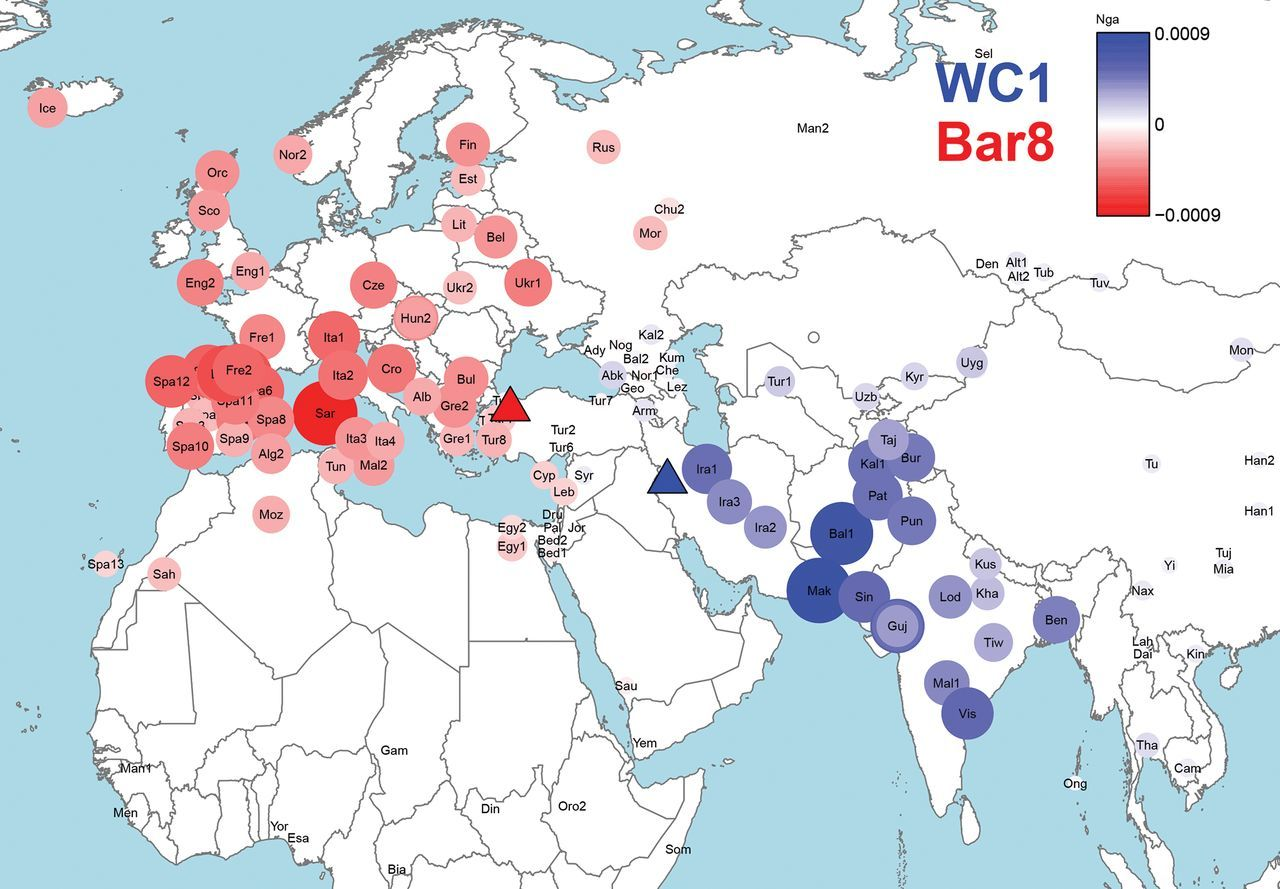
\includegraphics[width=1.0\textwidth]{../images/introduction/broushaki_haplotype_sharing.jpg}
    \caption{Map of differential haplotype sharing with present-day populations between WC1 (Iranian Farmer) and Bar8 (Anatolian Farmer) from Broushaki et al (2016) \cite{Broushaki2016a}. Bar8 copies relatively more from red populations and WC1 from blue populations.}
    \label{fig:broushaki_haplotype_sharing}
\end{figure}


The first use of ChromoPainter on ancient DNA was in the seminal paper of Lazaridis et al (2014) \cite{Lazaridis2014}. Through the generation of two high-coverage ancient genomes, they were the first to propose that most present-day Europeans can be modelled as a mixture of three ancestral populations. For the ChromoPainter analysis, they did not impute missing genotypes in the ancient samples, as the possible bias effects had yet to be studied; only positions with non-missing genotypes were retained. As the samples were of high coverage, this was not an issue, as 495,357 SNPs were kept. The the ability of fineSTRUCTURE to meaningfully cluster ancient individuals was confirmed by recapitulating previous results that identified different present-day European populations as being more closely related to Early Farmers and hunter-gatherers than others. 

In-between 2014 and the present-day, there have been approximately 31 studies which have used ChromoPainter on ancient samples (based on Web of Science search results). As of writing (September 2021), the study of Margaryan et al (2020) is the biggest so far to use ChromoPainter, with over 400 samples used \cite{margaryan2020population}. This study concluded that detecting structure within the dataset using `traditional' methods was not possible and so opted to use haplotype-based analyses on all samples above 0.5x mean depth. Another recent large study into the genomic history of the Roman Empire and surrounding regions leveraged ChromoPainter \cite{antonio2019ancient}.

More recently, ChromoPainter has been used to study aspects of archaic hominin ancestry in present-day humans \cite{JACOBS20191010, teixeira2021widespread}. Whilst ChromoPainter is not specifically designed to accurately estimate local ancestry, it is possible to infer identify potentially introgressed Denisovan regions of DNA by determining whether a haplotype which is more similar to the Denisovan genome than to a panel of sub-Saharan Africans. ChromoPainter has also been extended to studying the ancient DNA of non-human organisms such as bacteria \cite{Moodleye2015523118}. 

\subsubsection{Benchmarking ChromoPainter and imputation}

Many studies which have used ChromoPainter on ancient samples have performed tests and benchmarks to various degrees of detail. 

The first study to investigate the reliability of ChromoPainter on ancient DNA was Martiniano et al (2017) \cite{Martiniano2017}. Testing whether including imputed genotypes introduced bias towards particular present-day populations was key, as if it were the case, it may invalidate any results obtained. The authors estimated potential bias by plotting normal quantile-quantile plots of the copyvectors obtained from imputed (after downsampling to 2x coverage) and non-imputed markers. Whilst the differences in amount of copying differed by up to 14\%, most percentage differences were substantially lower and there was no evidence of structured bias towards or against particular geographic regions, with the authors concluding \blockquote{There is no strong evidence for systematic changes being caused by genotype imputation}.


The same study also investigated the impact of filtering genotypes based on genotype probabilities by creating two datasets, one containing filtered genotypes and without, and performing fineSTRUCTURE clustering on both. fineSTRUCTURE inferred 7 more clusters when using filtered genotypes; whilst this could be an indication of improved clustering resolution, it is hard to draw solid conclusions from these data. The overall number of fineSTRUCTURE clusters can not be seen as a direct measurement of performance; for example, the additional clusters inferred may simply be a result of the stochastic nature of MCMC sampling, and given only a single replicate of each test was performed, it is not possible to rule this out. Performing the same analysis on simulated data, where the population labels of individuals are known in advance, would be a more controlled test. 

Since the study of Martiniano et al, many papers which incorporated ChromoPainter analysis into studies of ancient DNA have included their own set of benchmarks. Antonio et al (2019) \cite{antonio2019ancient} tested imputation accuracy on an ancient sample (NE1) downsampled to different levels of coverage. However, this analysis was only performed on a single sample and the effect of imputation on the ChromoPainter process was not evaluated. Margaryan et al (2020) performed a downsampling test on two high coverage genomes down to 1x mean coverage and concluded that, whilst there was some suggestion that the 1x downsample tended to a more mixed ancestry profile, there was no evidence that incorrect ancestries have been inferred or that major changes in ancestries have occurred. 

Imputation is a necessary pre-processing step for ChromoPainter analysis on low-medium coverage ancient DNA samples for two primary reasons. Firstly, ChromoPainter does not allow for missing genotypes and so imputation is required to estimate missing genotypes. Secondly, whilst they are covered by reads, non-missing positions may still be low in coverage and thus require to be re-estimated, particularly when the true genotype is heterozygous. Therefore, it is important to determine to what extent it is possible to accurately impute genotypes at different levels of mean coverage. 

The accuracy of imputation on ancient samples has been tested in various studies \cite{Martiniano2017, hui2020evaluating, EmpiricalAncient}. There is difficulty in comparing the estimated accuracies between studies, however, due to differences in factors such as samples analyses, software used to call genotypes and impute samples, the regions analysed and filters applied. 

The most systematic and thorough evaluation of imputation in ancient genomes was performed by Hui et al (2020) \cite{hui2020evaluating}. This study noted that it is possible to impute using a one or two step approach and, through the use of downsampled genomes, showed that the two-step approach provides more accurate imputed genotypes. This study also showed that whilst most genotype likelihood callers (e.g. GATK, atlas) performed similarly well, atlas was preferred because of it's ability to model post-mortem damage (PMD) in ancient samples. Accordingly, I will use atlas to call genotype likelihoods in the rest of my thesis. 

It should be noted that the study only considered a single ancient genome (NE1) and it is therefore unclear how generalisable these results are to ancient samples of different ancestries. However, this study provided important benchmarks for many critical steps in the analysis of low coverage samples which had previously been missing from the literature, such as selection of a reference panel, the feasibility of local imputation and the effects of applying of pre and post imputation filters. One takeaway message was that it is possible to recover nine out of ten common (MAF $\geq$ 0.3) genotypes in a sample of 0.05x coverage. 

In Chapter 2 of my thesis, I will explore the effect of coverage on imputation and ChromoPainter performed on ancient DNA samples. 

\section{Issues and solution to low coverage data}

Low sequencing coverage is an issue which has plagued the field of ancient DNA since its inception. Compared to DNA obtained from present-day samples, ancient DNA samples typically have a much lower proportion of endogenous DNA, as DNA degrades over time from environmental factors. Therefore, when the DNA fragments are sequenced, relatively few of them will align to the human reference. 

The primary issue with low-coverage data is the increased uncertainty when calling diploid genotypes, particularly when the true genotype is heterozygous. Several methodological adaptations have been applied to existing methods in order to adapt them to low coverage ancient DNA. These approaches primarily attempt to circumvent making diploid genotype calls; for example, the previously mentioned strategy of pseudo-haploid genotype calling.

Alternatively, methods may avoid making diploid calls by working on genotype likelihoods. Genotype likelihoods represent a posterior estimate of the confidence of the three different genotypes at a bi-allelic locus, and thus allow the method to appropriately propogate that certainty throughout the analysis. A wide array of complex statistical approaches have been developed in order to accurately estimate the posterior genotype likelihoods. These approaches integrate factors such as sequencing-machine reported base-quality scores and estimates of read-mapping / sequencing errors \cite{McKenna2010}. Common methods to estimate likelihoods include the GATK model \cite{VanderAuwera2013}, SAMtools \cite{Li2009}, SOAPsnp \cite{Li2009a} and SYK model \cite{Kim2011}. Genotype likelihoods can either be estimated prior to the analysis from aligned reads (BAM files), using software such as ANGSD \cite{Korneliussen2014}, ATLAS \cite{Link2017} or GATK \cite{VanderAuwera2013}. Other softwares will take BAM files directly as input and estimate genotype likelihoods during the analysis process (e.g. STITCH \cite{Davies2016}). 

Once genotype likelihoods have been estimated, population level parameters such as inbreeding coefficients and $f_{st}$ can be estimated directly \cite{Korneliussen2014} with greater accuracy than direct genotype calls. Similarly, modifications of the ADMIXTURE \cite{Alexander2009} algorithm and PCA have been developed in order to analyse low coverage samples more effectively \cite{skotte2013estimating, zhang2021novel}. Recent advances have allowed the identification of 1st and 2nd-degree relatives from as low as 0.02x coverage samples \cite{fernandes2017identification, fernandes2021tkgwv2}. 

Several methods account for low-coverage data by jointly estimating ancient DNA specific confounding factors, such as contamination and  post-mortem damage, alongside the demographic parameter of interest \cite{Racimo2016}. For instance, Schraiber (2018) \cite{Schraiber2018} developed a novel maximum-likelihood approach which leverages information from different low-coverage samples from within the same population to infer population-level parameters, such as genetic continuity between ancient and modern populations.  
 
Viera et al (2016) developed a method (ngsF-HMM) to infer matching identical-by-descent (IBD) segments from low-coverage data \cite{Vieira2016}. To account for the uncertainty, all three genotype likelihoods are integrated over in order to estimate whether or not a genomic region is IBD given the likelihoods. This method showed that there is a substantial gain in power when likelihoods are used compared to genotype calls.  

In this thesis, I will attempt to mitigate any effects of low-coverage data on ChromoPainter analysis by implementing an approach similar to that of Viera et al (2016), which modifies the ChromoPainter algorithm to account for genotype likelihoods.


\section{Combining data from multiple chips}

An issue similar to that of low-coverage ancient DNA data stems from the development of a large number of different genotyping arrays. Different cohorts are genotyped on different arrays and sets of SNPs, as different SNPs have different characteristics, such as different frequencies in different populations and associations with different phenotypes. Whilst this has meant a wider variety of questions and populations can be studied, it also makes combining data from across different arrays potentially troublesome, as they often have a small overlap in the SNPs upon which they have been genotyped.

For example, in my thesis, I have worked with at least three genotyping arrays, referred to here as `Human Origins', `Hell Bus' and the UK Biobank. Often I have wanted to compare populations on different arrays, such as the African populations on the Human Origins array and UK Biobank individuals on the UK Biobank array. After merging the datasets, the overlap was small, only 70,000 SNPs. This is around an order of magnitude fewer SNPs than is analyse a typical ChromoPainter analysis. Having fewer SNPs may reduce power, as there are fewer pieces of information, and less linkage between each neighbouring SNP.

One solution to the issue of a small number of SNPs would be to impute the remaining SNPs using a reference panel and imputation algorithm such as Beagle \cite{Browning2016}. However, it is possible that imputation may cause a bias in the data. If missing genotypes are imputed incorrectly more often from one population than another, this will result in an increased, but spurious genetic similarity between the target and reference population. This may be a particular issue when analysing populations which are not well represented in imputation reference panels, such as non-Europeans. The nature and magnitude of this bias, however, is yet to be fully understood, particularly in the context of ChromoPainter.  

Therefore, this thesis will explore whether is it more desirable to impute the missing positions or to use use a smaller number of overlapping SNPs. Accordingly, in chapter 3 of this thesis, I will explore this question with a case study investigating African ancestry in the UK Biobank dataset. 
 
\section{Summary of thesis aims}

In this thesis I will explore the applicability of ChromoPainter to low-coverage ancient DNA samples and sparsely genotyped data resulting from merged genotype arrays. To do this, I will perform a series of tests on both real and simulated data from present-day and ancient samples and apply my findings to two novel (unpublished) datasets of ancient samples from Bavaria and Czechia. 

Specifically, in Chapter 2, I will perform downsampling simulations on five high-coverage ancient genomes to assess the impact of coverage on imputation, phasing and ChromoPainter analysis, and determine the feasibility of extracting haplotype information from sparsely genotyped data in practice. In Chapter 3, I will infer African ancestry across samples in the U.K. Biobank dataset, using sparsely genotyped data resulting from the merge of two different genotyping arrays. I will investigate the potential of using imputation to boost power to infer fine-scale ancestry signatures in U.K. Biobank participants, in terms of how closely related they are to individuals in reference data containing a large number of African ethnolinguistic groups. In Chapter 4, I will analyse unpublished ancient genome data from Bavaria, obtained by collaborators at Mainz University, exploring how genetic patterns varied from the Neolithic to the Medieval Era in a small geographic region. In Chapter 5, I will analyse unpublished ancient Slavic samples from Czechia, obtained by collaborators at Max Planck Institute for Evolutionary Anthropology, to assess the genetic relationships between Migration Era, Middle age and present-day Slavic-speaking peoples. Lastly, my concluding chapter will summarise my work and key findings, including my recommendations for future haplotype-based studies using low-coverage data and/or combining data from multiple SNP arrays.




